% Encoding: UTF-8

Die Bedeutung von Sicherheit in \enquote{cyber} Systemen und \enquote{physical} Systemen unterscheiden sich intrinsisch.
Um Klarheit zu schaffen wo diese Unterschiede liegen soll Sicherheit speziell für \gls{cps} definiert werden.

\subsection{Sicherheitsrelevante Eigenschaften von \glsentrytext{cps}}\label{subsec:definition}
% CIA triad (Fink) (WYX+10)
% Erweiterung von CIA: Veracity, Plausability (Gollman)
Unter Cybersicherheit versteht man im Allgemeinen Informationssicherheit.
Informationssicherheit kann man durch drei Eigenschaften von Systemen charakterisieren~\cite[,S.~2]{Cherdantseva2013,SFJ2017}:
\begin{itemize}[noitemsep,wide=0pt]
    \item \fb{Confidentiality} - Nur autorisierte Teilnehmer können auf die Infrastruktur zugreifen.
    \item \fb{Integrity} - Die Infrastruktur kann nur von autorisierten Teilnehmer verändert werden.
    \item \fb{Availability} - Die Infrastruktur ist für autorisierte Teilnehmer angemessen verfügbar.
\end{itemize}

Zwischen diesen drei Eigenschaften muss bei der Entwicklung ein sinnvolles Gleichgewicht gefunden werden.
\citeauthor{GK16} beschreiben, dass bei klassischen Cybersystemen der Fokus auf Confidentiality und bei \cps eher auf Availability liegt.
Dieser Fokus ist kritisch zu betrachten, wenn man die diversen Einsatzorte und sicherheitskritischen Anforderungen von \cps betrachtet.

Sie schlagen außerdem vor das CIA-Dreieck im Hinblick auf \cps durch die Eigenschaft ist Veracity (dt.~Richtigkeit) zu erweitern.
Ein System hat diese Eigenschaft genau dann, wenn Aussagen des Systems die Wahrhaftigkeit der  Wirklichkeit reflektieren.
Es muss also sichergestellt werden, dass Sensoren durch beispielsweise physische Maßnahmen (siehe Kapitel~\ref{subsec:physisch}) fälschungssicher sind.
Confidentiality und Integrity sind nicht ausreichend um die Richtigkeit von Informationen zu garantieren.
Die Richtigkeit beinhaltet auch, dass es nicht geleugnet werden darf bestimmte Aktionen ausgeführt zu haben \cite{NIST2013}.\todo{Wie zitiert man NIST?}
Veracity ist eine relativ starke Eigenschaft.
Deshalb kann man in Fällen, in denen diese nur schwer zu erreichen ist, zunächst auf Plausibility setzen.
Herbei hat ein System genau dann diese Eigenschaft, wenn Aussagen des Systems nicht zu weit von erwartbaren Werten abweichen.
Liefert ein Sensor beispielweise einen für physikalische Modelle unmögliche Wert, so ist dieser nicht plausibel und das System erreicht kann einen möglichen Angriff erkennen. \cite{GK16}

\citeauthor{WYX+10} und \citeauthor{SFJ2017} stimmen zu, dass eine Überprüfung auf die Richtigkeit von Informationen wichtig sind.
Sie erweitern das CIA-Dreieck zudem um die Eigenschaft der Authentizität zwischen Kommunikationspartnern.

\begin{figure}
    \centering
    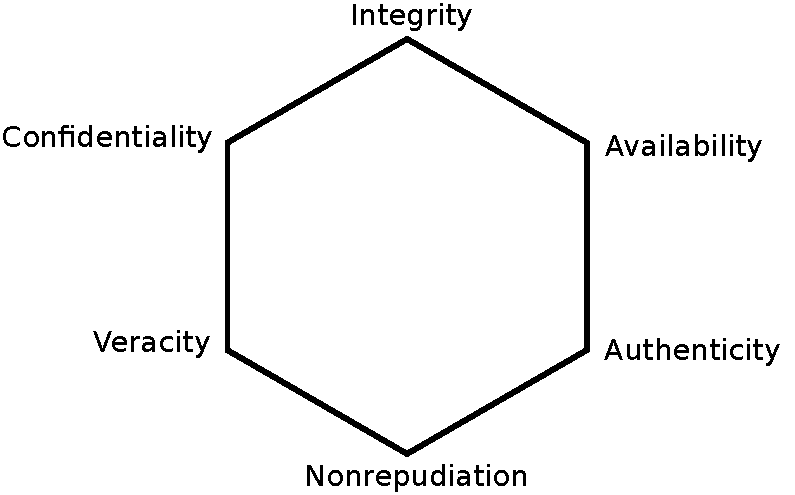
\includegraphics[width=0.5\textwidth]{triad}
    \caption{Erweitertes CIA-Dreieck}
    \label{fig:triad}
\end{figure}

Zusammenfassend kann man sagen, dass die Eigenschaften von Systemen aus der klassische Informationssicherheit nicht ausreichen um das oft komplexe Zusammenspiel von \enquote{physical} - und \enquote{cyber}-Einheiten abzusichern.
Bei \cps ist also sowohl die Richtigkeit von Informationen als auch die zweifelsfreie Identifikation zweier Parteien wichtig.
Deshalb sind Eigenschaften wie Veracity und Authenticity, wie in Abbildung~\ref{fig:triad} zu sehen ust, nötig um die Aspekte von \cps abzudecken.

% Definition (BG11)
% computer, information, network, communication, physical security
% Fingerprinting, Network Separation, End System Security (Gollman)

\subsection{Angreifergruppen}\label{subsec:angreifergruppen}
% Cyber-Kriminelle
% Verärgerte Mitarbeiter/Private Gründe
% Terroristen, Aktivisten, kriminelle Gruppen
% Staaten (Cardenas 2009, 2.) (WYX+10, II. C.)

Angriffe können von unterschiedlichen Gruppen aus unterschiedlichen Gründen ausgehen.
Im Folgenden sollen verschiedene Gruppen nach den Faktoren
\begin{enumerate*}[label=(\alph*),before=\unskip{: }, itemjoin={{; }}, itemjoin*={{, und }}]
    \item Angreifergruppe\label{factor:angreifergruppe}
    \item Angriffsziel\label{factor:target}
    \item Motiv\label{factor:motiv}
    \item Angriffsvektoren\label{factor:methode}
    \item Konsequenzen\label{factor:konsequenz}
\end{enumerate*} aufgezählt werden~\cite{HLL+17}.\todo{Aufzählung entfernen?}

Kriminelle Gruppen \ref{factor:angreifergruppe} haben oft Erpressung \ref{factor:motiv} als Ziel \cite{WYX+10}.
Dabei sind Cyberangriffe nur ein logischer nächster Schritt der Kriminellen, da diese weitaus günstiger, weniger riskant, nicht durch Entfernungen eingeschränkt und einfacher zu koordinieren und wiederholen sind. \cite{CAS+09}

Computerforensiker~\ref{factor:angreifergruppe} haben nicht unbedingt als Ziel selbst ein System zu beschädigen.
Zum einen kann das Finden von Lücken aber auch als Ziel haben, diese unter bestimmten Auflagen offen zulegen, um diese zu schließen zu können~\ref{factor:motiv}. \todo{Zitat fehlt}
Zum anderen kann eine Schadsoftware verkaufen werden~\ref{factor:motiv}. \todo{Zitat fehlt}

Unzufriedene Mitarbeiter~\ref{factor:angreifergruppe} eines Unternehmens haben viel Wissen über dessen Infrastruktur.
Das Motiv kann liegt hierbei bei der Schädigung des Unternehmens~\ref{factor:motiv}.
Zudem existiert eventuell Zugriff auf das System, sodass überhaupt kein Umgehen von Sicherheitsmechanismen notwendig ist~\ref{factor:methode}.~\cite{CAS+09,WYX+10}

Aktivistische Gruppierungen~\ref{factor:angreifergruppe} zielen oft auf kritische \cps~\ref{factor:target}, wie beispielsweise Kernkraftwerke oder \gls{scada} Systemen in Fabriken, ab, um diese zu manipulieren \cite{CAS+09,HLL+17}. \todo{Spionage?}
Damit dies erreicht werden kann existiert die Möglichkeit Forensiker oder Insider zu engagieren~\ref{factor:methode}.~\cite{WYX+10}

Staaten~\ref{factor:angreifergruppe} können politisches und militärisches Interesse~\ref{factor:motiv} daran haben Infrastruktur innerhalb oder außerhalb des Staatsgebiets~\ref{factor:target} anzugreifen \cite{CAS+09}, um diese zu zu sabotieren oder auszuspionieren.
Auch hier werden Forensiker oder Insider zu engagieren~\ref{factor:methode}.

Das Wissen über den Angreifer und dessen Motivation kann maßgeblich bei der Wahl und der Strategie der Gegenmaßnahmen helfen.
Zudem können Gefahrenmodelle und detailliertere Angriffsszenarien entworfen werden (siehe Kapitel~\ref{sec:angriffszenarien}).


\subsection{\glsentrytext{cps} als Angriffsziel}\label{subsec:angriffsziel}
\todo{Noch sehr unzufrieden mit diesem Kapitel, Eventuell anderer Aufbau: Problem -> Beispiel}
Es gibt eine Vielzahl von Anwendungen für \cps, wie beispielsweise industrielle Kontrollsysteme, intelligente Stromnetze, medizinische Geräte und intelligente Autos~\cite{HLL+17}.
\todo{Acronym ICS, ICCP, DNP3, Modbus}
Hierbei sind die unterschiedlichsten Protokolle und Busse zur Kommunikation.
ICCP, Modbus oder auch DNP3, die Verwendung bei Industrial Control Systems und intelligenten Stromnetze finden~\cite{HLL+17}, implementieren keine Verschlüsselung oder Authentifizierung \cite{HUM 124,HUM 38,HUM 69}, wodurch Lauschangriffe (siehe Kapitel~\ref{subsec:lauschen}) möglich sind.
Es ist also wichtig offene Protokolle, wie ICCP oder TCP/IP, zu verwenden, sodass man Grundlegende Eigenschaften der Confidentiality und Authenticity bei einem \cps bestimmen kann und falls nötig diese nachrüsten kann.

Bei medizinischen Geräten ist eine kabellose Verbindung oft notwendig~\cite{HLL+17}, da Aktualisierungen über ein Kabel nur schwer umzusetzen sind.
Besonders in diesem Bereich sollte das Bewusstsein für Sicherheit wachsen, da direkt Menschenleben und deren Privatsphäre, davon abhängen wie sicher diese Systeme sind.

Durch diese Vielfalt an Kommunikationsmöglichkeiten und der Heterogenität der einzelnen Komponenten gibt es auch eine dementsprechend große Angriffsfläche~\cite{HLL+17}.
Zudem wird bei der Entwicklung oft versucht durch proprietäre Protokolle und deren Obskurität Sicherheit zu gewährleiten~\cite{HLL+17,SJT2008}\todo{cite NIST}.

% Die Umgebung des \cps ist meist vor der Entwicklung noch nicht bekannt oder wird ignoriert~\cite{CAS08,Ericsson2010}.

% IoT (FPA+18) (YWY+17)
% Security Considerations in Cloud (SPB+16)

\begin{figure}
    \centering
    \begin{subfigure}[b]{0.3\textwidth}
        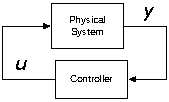
\includegraphics[width=\textwidth]{abstrakt}
        \caption{Ohne Angriffspunkte}
        \label{fig:abstrakt}
    \end{subfigure}
    \qquad
    \begin{subfigure}[b]{0.4\textwidth}
        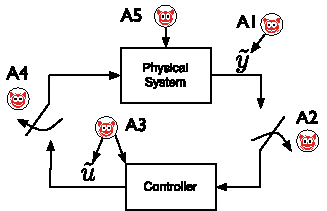
\includegraphics[width=\textwidth]{attack_points}
        \caption{Mit Angriffspunkten}
        \label{fig:attack_points}
    \end{subfigure}
    \caption{Abstraktion eines \cps~\cite{CAS08}}
\end{figure}

In Abbildung~\ref{fig:abstrakt} ist eine abstrakte Darstellung eines \cps zu sehen.
Der Controller sendet Befehle über u and das \enquote{physical}-System.
Dieses wiederum schickt Resultate oder Sensorwerte an das \enquote{cyber}-System.
In Abbildung~\ref{fig:attack_points} sind mögliche Angriffspunkte dargestellt.
Hierbei stellen A1 und A2 Täuschungsangriffe dar (siehe Kapitel~\ref{subsec:tauschung}), A4 und A2 \gls{dos} (siehe Kapitel ~\ref{subsec:dos}) und A5 einen physischen Angriff (siehe Kapitel~\ref{subsec:tauschung}).
Diese und noch weitere Szenarien sollen im folgenden Kapitel genauer ausgeführt werden.



% Survey: medial, IoT, smart grid, power plant (Humayed)
